%----------------------------------------------------------------------------------------
%   Доорх хэсгийг өөрчлөх шаардлагагүй
%----------------------------------------------------------------------------------------
%!TEX TS-program = xelatex
%!TEX encoding = UTF-8 Unicode
\documentclass[12pt,A4]{report}

\usepackage{fontspec,xltxtra,xunicode}
\setmainfont[Ligatures=TeX]{Times New Roman}
\setsansfont{Arial}

% \usepackage[utf8x]{inputenc}
% \usepackage[mongolian]{babel}
%\usepackage{natbib}
\usepackage{geometry}
%\usepackage{fancyheadings} fancyheadings is obsolete: replaced by fancyhdr. JL
\usepackage{fancyhdr}
\usepackage{float}
\usepackage{afterpage}
\usepackage{graphicx}
\usepackage{amsmath,amssymb,amsbsy}
\usepackage{dcolumn,array}
\usepackage{tocloft}
\usepackage{dics}
\usepackage{nomencl}
\usepackage{upgreek}
\newcommand{\argmin}{\arg\!\min}
\usepackage{mathtools}
\usepackage[hidelinks]{hyperref}
\usepackage{bookmark}

\usepackage{algorithm}
\usepackage{algpseudocode}

\usepackage{listings}
\DeclarePairedDelimiter\abs{\lvert}{\rvert}%
\makeatletter
\usepackage{caption}
\captionsetup[table]{belowskip=0.5pt}
\usepackage{subfiles}

\usepackage{listings}
\renewcommand{\lstlistingname}{Код}
\renewcommand{\lstlistlistingname}{\lstlistingname ын жагсаалт}

\usepackage{color}
\definecolor{codegreen}{rgb}{0,0.6,0}
\definecolor{codegray}{rgb}{0.5,0.5,0.5}
\definecolor{codepurple}{rgb}{0.58,0,0.82}
\definecolor{backcolour}{rgb}{0.99,0.99,0.99}
\definecolor{darkgray}{rgb}{0.99,0.103,0.105}
\definecolor{purple}{rgb}{0.128,0,0.128}
\usepackage{longtable}
\usepackage{booktabs}
\lstdefinestyle{mystyle}{
    basicstyle=\ttfamily\small,
    backgroundcolor=\color{backcolour},   
    commentstyle=\color{codegreen},
    keywordstyle=\color{magenta},
    numberstyle=\tiny\color{codegray},
    stringstyle=\color{codepurple},
    %basicstyle=\footnotesize,
    breakatwhitespace=false,         
    breaklines=true,                 
    captionpos=b,                    
    keepspaces=false,                 
    numbers=left,                    
    numbersep=10pt,                  
    showspaces=false,                
    showstringspaces=true,
    showtabs=false,                  
    tabsize=2
}
 
 %define Javascript language
\lstdefinelanguage{JavaScript}{
keywords={typeof, new, true, false, catch, function, return, null, catch, switch, var, if, in, while, do, else, case, break},
keywordstyle=\color{blue}\bfseries,
ndkeywords={class, export, boolean, throw, implements, import, this},
ndkeywordstyle=\color{darkgray}\bfseries,
identifierstyle=\color{black},
sensitive=false,
comment=[l]{//},
morecomment=[s]{/*}{*/},
commentstyle=\color{purple}\ttfamily,
stringstyle=\color{red}\ttfamily,
morestring=[b]',
morestring=[b]"
}
 
\lstset{
language=JavaScript,
extendedchars=true,
basicstyle=\footnotesize\ttfamily,
showstringspaces=false,
showspaces=false,
numbers=left,
numberstyle=\footnotesize,
numbersep=9pt,
tabsize=2,
breaklines=true,
showtabs=false,
captionpos=b
}
 
\lstset{style=mystyle, label=DescriptiveLabel} 


\let\oldabs\abs
\def\abs{\@ifstar{\oldabs}{\oldabs*}}
\makenomenclature
\begin{document}


%----------------------------------------------------------------------------------------
%   Өөрийн мэдээллээ оруулах хэсэг
%----------------------------------------------------------------------------------------

% Дипломийн ажлын сэдэв
\title{Програм хангамжийн зохиомжийн үлгэр загварууд ба түүний хэрэглээ}
% Дипломын ажлын англи нэр
\titleEng{Software design patterns and its application}
% Өөрийн овог нэрийг бүтнээр нь бичнэ
\author{Цэдэн-Ишийн Биндэрцэцэг}
% Өөрийн овгийн эхний үсэг нэрээ бичнэ
\authorShort{Ц. Биндэрцэцэг}
% Удирдагчийн зэрэг цол овгийн эхний үсэг нэр
\supervisor{Х. Ганзориг}
% Хамтарсан удирдагчийн зэрэг цол овгийн эхний үсэг нэр
\cosupervisor{Б. Батням}

% СиСи дугаар 
\sisiId{22B1NUM0027}
% Их сургуулийн нэр
\university{МОНГОЛ УЛСЫН ИХ СУРГУУЛЬ}
% Бүрэлдэхүүн сургуулийн нэр
\faculty{МЭДЭЭЛЛИЙН ТЕХНОЛОГИ, ЭЛЕКТРОНИКИЙН СУРГУУЛЬ}
% Тэнхимийн нэр
\department{МЭДЭЭЛЭЛ, КОМПЬЮТЕРИЙН УХААНЫ ТЭНХИМ}
% Зэргийн нэр
\degreeName{Үйлдвэрлэлийн дадлагын тайлан}
% Суралцаж буй хөтөлбөрийн нэр
\programeName{Програм Хангамж (D061302)}
% Хэвлэгдсэн газар
\cityName{Улаанбаатар хот}
% Хэвлэгдсэн огноо
\gradyear{2025 оны 9 сар}
% Дадлага хийж байгаа газрын  нэр
% \company{Монгол Ай Ди}
% Дадлага хийж байгаа газрын англи нэр
% \companyEng{Mongol ID}

%----------------------------------------------------------------------------------------
%   Доорх хэсгийг өөрчлөх шаардлагагүй
%----------------------------------------------------------------------------------------
%----------------------Нүүр хуудастай хамаатай зүйлс----------------------------
\pagenumbering{roman}
\makefrontpage
\maketitle

\doublespace

% Decleration
\begin{huge}
\textbf{Зохиогчийн баталгаа}
\end{huge} \\ \ \\ 
\doublespace
Миний бие \@author \ нь "\@title" \ сэдэвтэй дадлагын ажлыг гүйцэтгэсэн болохыг зарлаж дараах зүйлсийг баталж байна:
\begin{itemize}
\item Энэхүү ажлын аль нэг хэсгийг эсвэл бүхлээр нь ямар нэг их, дээд сургуулийн зэрэг горилохоор оруулаагүй болно.
\item Бусдын хийсэн ажлаас хуулбарлаагүй, ашигласан бол ишлэл, зүүлт хийсэн.
\item Ажлыг би өөрөө (хамтарч) хийсэн ба миний хийсэн ажил, үзүүлсэн дэмжлэгийг дадлагын ажилд тодорхой тусгасан. 
\item Ажилд тусалсан бүх эх сурвалжид талархаж байна.  
\end{itemize} 
\ 

Гарын үсэг: \underline{\hspace{5cm}}

Огноо: 	\ \ \underline{\hspace{3cm}}

\newpage
%----------------------------------------------------------------------------------------
% Хавсралтын нэр. Хавсралт гэдэг үг агуулахгүй
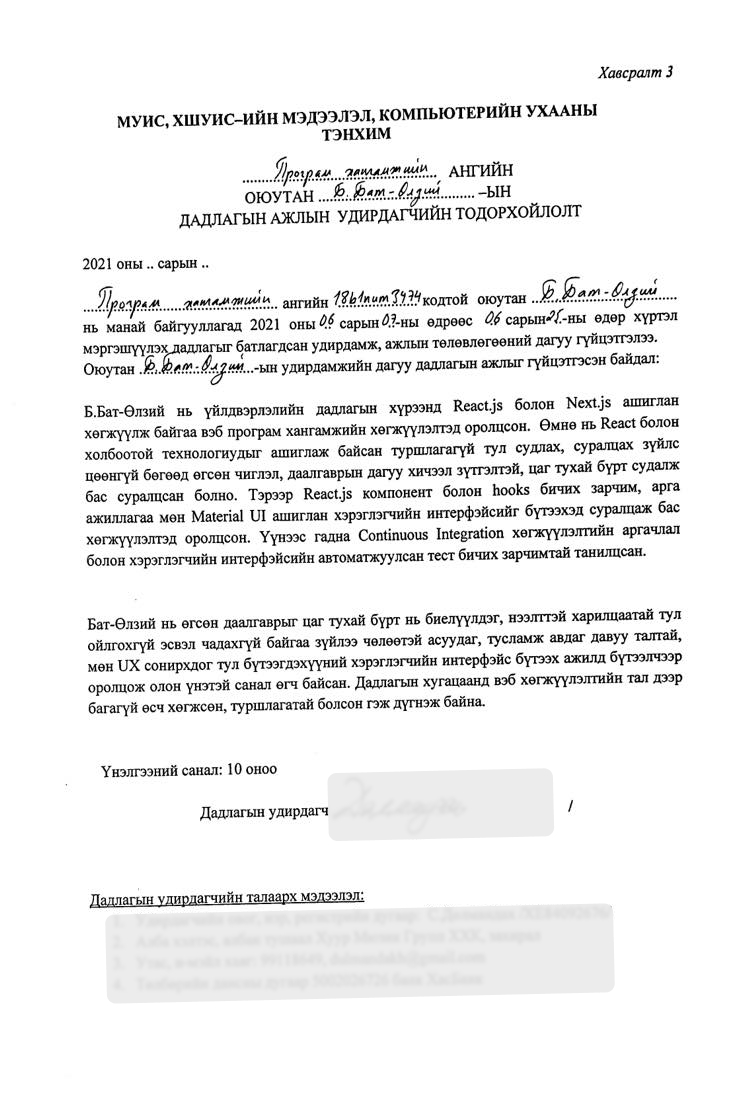
\includegraphics[width=14cm]{images/review.jpg}
%----------------------------------------------------------------------------------------
\newpage
%----------------------------------------------------------------------------------------
%   Агуулгын хэсэг
\begin{table}[h]
\caption{Дадлагын төлөвлөгөө}
\begin{tabular}{|p{0.5cm}|p{8cm}|l|l|p{3cm}|}
\hline
\text{№} & \text{Гүйцэтгэх ажил} & \text{Хугацаа} & \text{Биелэлт} & Удирдагчийн үнэлгээ \\ \hline
1 & Програм хангамжийн үлгэр загваруудын тухай судлах & 08/11 - 08/15 & дууссан & \\ \hline
2 & Жава, Spring Boot, Spring MVC технологиудын тухай судлах & 08/11 - 08/15 & дууссан & \\ \hline
3 & Auftragsverwaltung системийн классын диаграмыг гаргах & 08/12 - 08/14 & дууссан & \\ \hline
4 & Auftragsverwaltung систем дээр ашигласан зохиомжийн үлгэр загваруудыг олж тогтоох & 08/14 - 08/18 & дууссан & \\ \hline
5 & МУИС-ын дипломын ажлыг удирдах системийн шаардлагатай танилцах  & 08/18 & дууссан & \\ \hline
6 & Уг шаардлагын дагуу системийн зохиомжийг загварчлах & 08/18 - 08/20 & дууссан & \\ \hline
7 & Системийн хэрэгжүүлэлтийг Жава технологи ашиглан гүйцэтгэх & 08/20 - 08/22 & дуусаагүй & \\ \hline
8 & Банкны Excel хуулгыг боловсруулах модулийн шинжилгээг гүйцэтгэх & 08/22 & дууссан & \\ \hline
9 & Уг шаардлага дээрээ үндэслэн зохиомж болон архитектурыг гаргах & 08/23 - 08/24 & дууссан & \\ \hline
10 & Уг зохиомжийн дагуу модулийн хэрэгжүүлэлтийг Spring Boot фреймворк ашиглан гүйцэтгэх & 08/25 - 08/29 & дууссан & \\ \hline
11 & Модулийг JUnit санг ашиглан тестлэх & 08/27 - 08/30 & дууссан & \\ \hline
\end{tabular}
\end{table}
%----------------------------------------------------------------------------------------

% Гарчгийг автоматаар оруулна
\setcounter{tocdepth}{1}
\tableofcontents

% Зургийн жагсаалтыг автоматаар оруулна
\listoffigures

% Хүснэгтийн жагсаалтыг автоматаар оруулна
\listoftables

% Кодын жагсаалтыг автоматаар оруулна
\lstlistoflistings

\newpage
%% \addtocontents{lof}{Зураг~\hfill Хуудас \par}
\newpage
%% \addtocontents{lot}{Хүснэгт~\hfill Хуудас \par}

\renewcommand{\cftlabel}{Зураг}


\doublespace
\pagenumbering{arabic}

\begin{abstract}
 \quad \quad \quad Миний бие \@author \ нь үйлдвэрлэлийн дадлагын 3 долоо хоногийн хугацаанд програм хангамжийн зохиомжийн үлгэр загваруудын хүрээнд урвуу инженерчлэл -ийн аргачлал, Жава, Spring Boot, Spring MVC гэсэн технологиуд дээр голчлон ажилласан ба уг технологиуд ямар шалтгаанаар үүссэн, хөгжүүлэлтийн ямар арга барил ашигладаг, компаниуд хэрхэн үүн дээр хөгжүүлэлт хийж эцсийн бүтээгдэхүүнийг гаргадаг талаар судлах -ын тулд Java Spring Boot фрэймворк ашигладаг компани болох "Монгол Ай Ди" байгууллагыг сонгон авч мэргэжлийн дадлагаа гүйцэтгэлээ.

  \quad \quad \quad Дадлагын эхний долоо хоногт би бараа захиалгийг зохицуулах "Auftragsverwaltung" систем дээр урвуу инженерчлэлийн аргачлал ашиглан зохиомжийн үлгэр загваруудыг уг системд хэрхэн ашигласан байгааг олж тогтоосон. Үүний дараа МУИС-ийн дипломын ажлыг удирдах системийн шаардлагийн дагуу системийн зохиомжийг гаргаж, уг зохиомж дээр үндэс -лэн системийг Жава технологи ашиглан хэрэгжүүллээ.

  \quad \quad \quad Дадлагын сүүлийн долоо хоногт Монгол Ай Ди компанийн хөгжүүлж буй дотоод зээлийн системийн асуудал шийдвэрлэх хэсэг дээр ажилласан. Миний хариуцаж авсан модуль нь хэрэглэгчийн дансны Excel хуулгыг сервер рүү ачаалж, хуулга доторх өгөгдлийг боловсруу -лан системийн өгөгдлийн сантай уялдуулж, хэрэглэгчийн зээлийн мэдээллийг шинэчлэх үүрэгтэй. Уг модуль дээр ажиллахын тулд би Spring Boot, Spring MVC технологийн талаар судалгаа хийж, компанийн хөгжүүлэлтийн арга барилтай танилцаж, өгөгдсөн асуудлыг шийд -вэрлэлээ.
  
  % \quad \quad \textbf{Зорилго} React болон Next.js технологийн талаар судалж, компанийн хөгжүүлэлтийн арга барилтай танилцах
  
  % \quad \quad \textbf{Зорилт} Удирдагчийн зааварчилгааны дагуу алхам алхмаар судалгаа хийж өгсөн шаардлагын хүрээнд хэрэгжүүлэлт хийх
\end{abstract}


% \begin{table}[h]
\caption{Дадлагын төлөвлөгөө}
\begin{tabular}{|p{0.5cm}|p{8cm}|l|l|p{3cm}|}
\hline
\text{№} & \text{Гүйцэтгэх ажил} & \text{Хугацаа} & \text{Биелэлт} & Удирдагчийн үнэлгээ \\ \hline
1 & Программ хангамжийн үлгэр загваруудын тухай судлах & 08/11 - 08/15 & дууссан & \\ \hline
2 & Жава, Spring Boot, Spring MVC технологиудын тухай судлах & 08/11 - 08/15 & дууссан & \\ \hline
3 & Auftragsverwaltung системийн классын диаграмыг гаргах & 08/12 - 08/14 & дууссан & \\ \hline
4 & Auftragsverwaltung систем дээр ашигласан зохиомжийн үлгэр загваруудыг олж тогтоох & 08/14 - 08/18 & дууссан & \\ \hline
5 & МУИС-ын дипломын ажлыг удирдах системийн шаардлагатай танилцах  & 08/18 & дууссан & \\ \hline
6 & Уг шаардлагын дагуу системийн зохиомжийг загварчлах & 08/18 - 08/20 & дууссан & \\ \hline
7 & Системийн хэрэгжүүлэлтийг Жава технологи ашиглан гүйцэтгэх & 08/20 - 08/22 & дуусаагүй & \\ \hline
8 & Банкны Excel хуулгыг боловсруулах модулийн шинжилгээг гүйцэтгэх & 08/22 & дууссан & \\ \hline
9 & Уг шаардлага дээрээ үндэслэн зохиомж болон архитектурыг гаргах & 08/23 - 08/24 & дууссан & \\ \hline
10 & Уг зохиомжийн дагуу модулийн хэрэгжүүлэлтийг Spring Boot фреймворк ашиглан гүйцэтгэх & 08/25 - 08/29 & дууссан & \\ \hline
11 & Модулийг JUnit санг ашиглан тестлэх & 08/27 - 08/30 & дууссан & \\ \hline
\end{tabular}
\end{table}


\addcontentsline{toc}{part}{БҮЛГҮҮД}

\chapter{Байгууллагын танилцуулга}
\subfile{chapters/introduction}

\chapter{Зорилго ба зорилт}
\subfile{chapters/goal}

\chapter{Онолын судалгаа}
\subfile{chapters/research}

\chapter{Дадлагын бэлтгэл ажил}
\subfile{chapters/reverse}

\chapter{Системийн шинжилгээ}
\subfile{chapters/analysis}

\chapter{Системийн зохиомж}
\subfile{chapters/design}

\chapter{Ашигласан технологи}
\subfile{chapters/technologies}

\chapter{Хэрэгжүүлэлт}
\subfile{chapters/implementation}

\chapter{Дүгнэлт}
\subfile{chapters/conclusion.tex}

%----------------------------------------------------------------------------------------
%   Дипломын номзүй, хавсралтын хэсэг эндээс эхэлнэ
%----------------------------------------------------------------------------------------

\singlespace
\addcontentsline{toc}{part}{НОМ ЗҮЙ}
\begin{thebibliography}{99}
	% Ашигласан материалыг эндээс оруулна
	\bibitem{declarative}
	Declarative програмчлал болон Imperative програмчлалын ялгаа
	\\\url{https://codeburst.io/declarative-vs-imperative-programming-a8a7c93d9ad2}
	\bibitem{material-ui-beta}
	Material-ui Beta v5 хувилбарын Card ашиглах заавар
	\\\url{https://next.material-ui.com/api/card/}
\end{thebibliography}



%----------------------------------------------------------------------------------------
%   Хавсралтууд эндээс эхэлнэ
%----------------------------------------------------------------------------------------
\appendix
\addcontentsline{toc}{part}{ХАВСРАЛТ}

% Хавсралтын нэр. Хавсралт гэдэг үг агуулахгүй
\chapter{Удирдагчийн үнэлгээ}
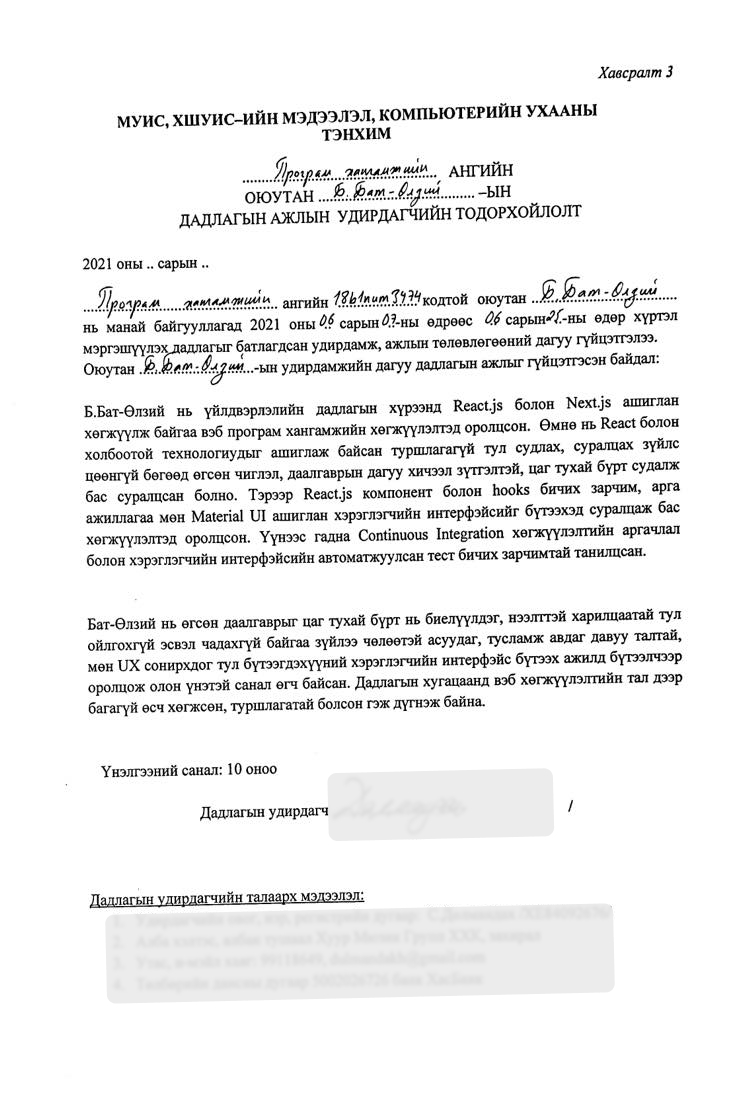
\includegraphics[width=14cm]{images/review.jpg}

\chapter{Конвенц}
\subfile{chapters/appendixtable.tex}
% Хавсралтын нэр. Хавсралт гэдэг үг агуулахгүй
\chapter{Кодын хэрэгжүүлэлт}

\section{Форм}

\subsection{useReducer болон React-Select сан ашигласан байдал}
\begin{lstlisting}[language=Javascript, frame=single]
import { useState, useReducer } from "react";
import Head from "next/head";
import styles from "../styles/Home.module.css";
import Select from "react-select";
import address from "../data/address";

const SET_CITY = "city";
const SET_DISTRICT = "district";
const SET_WARD = "ward";

const reducer = (state, action) => {
  switch (action.type) {
    case SET_CITY:
      return {
        city: action.index,
        district: null,
        ward: null,
      };
    case SET_DISTRICT:
      return {
        ...state,
        district: action.index,
        ward: null,
      };
    case SET_WARD:
      return {
        ...state,
        ward: action.index,
      };
    default:
      return state;
  }
};

export default function Home() {
  const [state, dispatch] = useReducer(reducer, {
    city: null,
    district: null,
    ward: null,
  });

  const handleChange = (index, type) => {
    dispatch({ type: type, index });
  };

  const register = (e) => {
    e.preventDefault();
    console.log(state);
  };

  return (
    <div className={styles.container}>
      <Head>
        <title>Create Next App</title>
      </Head>

      <main className={styles.main}>
        <div>
          <form className={styles.grid} onSubmit={register}>
            <label>
              <p>Хот/Аймаг:</p>
              <Select
                value={address.map((i, index) => ({ ...i, index }))[state.city]}
                onChange={(e) => handleChange(e.index, SET_CITY)}
                options={address.map((i, index) => ({ ...i, index }))}
                getOptionLabel={(option) => option.name}
                getOptionValue={(option) => option.index}
                placeholder="Сонгох"
              />
            </label>

            <label>
              <p>Сум/Дүүрэг:</p>
              <Select
                value={
                  state.district != null
                    ? address[state.city].districts.map((i, index) => ({
                        ...i,
                        index,
                      }))[state.district]
                    : []
                }
                onChange={(e) => handleChange(e.index, SET_DISTRICT)}
                options={
                  state.city != null
                    ? address[state.city].districts.map((i, index) => ({
                        ...i,
                        index,
                      }))
                    : []
                }
                getOptionLabel={(option) => option.name}
                getOptionValue={(option) => option.index}
                placeholder="Сонгох"
              />
            </label>

            <label>
              <p>Баг/Хороо:</p>
              <Select
                value={
                  state.ward != null
                    ? address[state.city].districts[state.district].wards.map(
                        (i, index) => ({ ...i, index })
                      )[state.ward]
                    : []
                }
                onChange={(e) => handleChange(e.index, SET_WARD)}
                options={
                  state.district != null
                    ? address[state.city].districts[state.district].wards.map(
                        (i, index) => ({ ...i, index })
                      )
                    : []
                }
                getOptionLabel={(option) => option.name}
                getOptionValue={(option) => option.index}
                placeholder="Сонгох"
              />
            </label>
            <button className={styles.registerBtn}>Бүртгүүлэх</button>
          </form>
        </div>
      </main>
    </div>
  );
}
\end{lstlisting}

\subsection{Functional component дээр state ашигласан байдал}

\begin{lstlisting}[language=Javascript, frame=single]
import { useEffect, useState } from "react";
import Head from "next/head";
import styles from "../styles/Home.module.css";
import axios from "axios";
import useForm from "../utils/useForm";

const fetchData = (url) => {
  //get data from next.js api
  return axios
    .get(`http://localhost:3000/api/${url}`)
    .then((res) => {
      const results = res.data;
      return results;
    })
    .catch((err) => {
      console.error(err);
    });
};

export default function Home() {
  const [values, handleChange] = useForm();
  const [data, setData] = useState({
    cities: [],
    districts: [],
    wards: [],
  });

  useEffect(() => {
    fetchData(`cities`)
      .then((res) => {
        setData({ ...data, cities: res });
      })
      .catch((err) => {
        console.error(err);
      });
  }, []);

  const register = (e) => {
    e.preventDefault();
    console.log(values);
  };

  const handleSelect = (id, type) => {
    if (type == "city") {
      fetchData(`cities/${id}`)
        .then((res) => {
          setData({ ...data, districts: res, wards: [] }); //set districts and clear wards data
        })
        .catch((err) => {
          console.error(err);
        });
    } else if (type == "district") {
      //get wards
      fetchData(`cities/${values.city}/${id}`)
        .then((res) => {
          setData({ ...data, wards: res });
        })
        .catch((err) => {
          console.error(err);
        });
    }
  };

  const OptionItems = (props) => {
    const options = props.items.map((item) => {
      return (
        <option key={item.id} value={item.id}>
          {item.name}
        </option>
      );
    });

    return options;
  };

  return (
    <div className={styles.container}>
      <Head>
        <title>Create Next App</title>
      </Head>

      <main className={styles.main}>
        <div>
          <form className={styles.grid} onSubmit={register}>
            <label>
              Хот/Аймаг:
              <select
                value={values.city}
                defaultValue="default"
                name="city"
                onChange={(e) => {
                  handleChange(e.target.name, e.target.value);
                  handleSelect(e.target.value, "city");
                }}
              >
                <option value="default" hidden>
                  Хот/Аймаг
                </option>

                {data.cities.length > 0 ? (
                  <OptionItems items={data.cities} />
                ) : null}

                {/* {data.cities.map((item) => {
                  return (
                    <option key={item.id} value={item.name}>
                      {item.name}
                    </option>
                  );
                })} */}
              </select>
            </label>

            <label>
              Сум/Дүүрэг:
              <select
                value={values.district}
                defaultValue="default"
                name="district"
                onChange={(e) => {
                  handleChange(e.target.name, e.target.value);
                  handleSelect(e.target.value, "district");
                }}
              >
                <option value="default" hidden>
                  Сум/Дүүрэг
                </option>
                {data.districts.length > 0 ? (
                  <OptionItems items={data.districts} />
                ) : null}
              </select>
            </label>

            <label>
              Баг/Хороо:
              <select
                value={values.ward}
                defaultValue="default"
                name="ward"
                onChange={(e) => {
                  handleChange(e.target.name, e.target.value);
                }}
              >
                <option value="default" hidden>
                  Баг/Хороо
                </option>
                {data.wards.length > 0 ? (
                  <OptionItems items={data.wards} />
                ) : null}
              </select>
            </label>
            <button style={{ margin: "5px" }}>Бүртгүүлэх</button>
          </form>
        </div>
      </main>
    </div>
  );
}
\end{lstlisting}

\section{Toast компонент}

\subsection{Toast/context.tsx - Context үүсгэх}
\begin{lstlisting}[language=Javascript, frame=single]
import { createContext, useReducer } from "react";

import { ActionType } from "types";

export interface ToastType {
  id?: string;
  message: string;
  type: "success" | "info" | "warning" | "error";
  duration?: number;
}

export const ACTION_TOAST = "TOAST";
export const ACTION_RESET = "RESET";
export const ACTION_CLEAR = "CLEAR";

export const INITIAL_STATE: { toasts: ToastType[] } = {
  toasts: [],
};

type Actions =
  | (ActionType<typeof ACTION_TOAST> & { toast: ToastType })
  | ActionType<typeof ACTION_RESET>
  | (ActionType<typeof ACTION_CLEAR> & { id: string });

export const ToastContext = createContext(null);
ToastContext.displayName = "ToastContext";
export const ToastControlContext = createContext(null);
ToastControlContext.displayName = "ToastControlContext";

function toast(state: typeof INITIAL_STATE, toast: ToastType): typeof state {
  return {
    ...state,
    toasts: [...state.toasts, toast],
  };
}

function clear(state: typeof INITIAL_STATE, toastId: string): typeof state {
  return {
    ...state,
    toasts: state.toasts.filter((toast) => toast.id !== toastId),
  };
}

function reducer(state = INITIAL_STATE, action: Actions): typeof state {
  switch (action.type) {
    case ACTION_TOAST:
      return toast(state, action.toast);
    case ACTION_RESET:
      return INITIAL_STATE;
    case ACTION_CLEAR:
      return clear(state, action.id);
    default:
      return state;
  }
}

export const ToastProvider = ({ children }) => {
  const [state, dispatch] = useReducer(reducer, INITIAL_STATE);

  return (
    <ToastContext.Provider value={state}>
      <ToastControlContext.Provider value={dispatch}>
        {children}
      </ToastControlContext.Provider>
    </ToastContext.Provider>
  );
};
\end{lstlisting}

\subsection{Toast/hooks.ts - Custom hook бичих}

\begin{lstlisting}[language=Javascript, frame=single]
import { useCallback, useContext, useMemo } from "react";

import {
  ACTION_CLEAR,
  ACTION_TOAST,
  ACTION_RESET,
  ToastContext,
  ToastControlContext,
  ToastType,
} from "./context";

function generateToastId() {
  return Math.random().toString(36).substr(2, 9);
}

export function useToast() {
  const state = useContext(ToastContext);
  if (!state) throw new TypeError("Please use within ToastProvider");
  return state;
}

export function useToastControl() {
  const dispatch = useContext(ToastControlContext);
  if (!dispatch) throw new TypeError("Please use within ToastProvider");

  const reset = useCallback(() => dispatch({ type: ACTION_RESET }), [dispatch]);

  const toast = useCallback(
    (toast: ToastType) => {
      const toastId = generateToastId();

      dispatch({ toast: { ...toast, id: toastId }, type: ACTION_TOAST });

      setTimeout(() => {
        dispatch({ id: toastId, type: ACTION_CLEAR });
      }, toast.duration || 4000);
    },
    [dispatch]
  );

  return useMemo(() => {
    return { reset, toast };
  }, [toast, reset]);
}
\end{lstlisting}

\subsection{Toast/index.ts}

\begin{lstlisting}[language=Javascript, frame=single]
export * from "./Toast";
export * from "./context";
export * from "./hooks";

\end{lstlisting}

\subsection{Toast/Toast.tsx - Үндсэн Toast компонент}

\begin{lstlisting}[language=Javascript, frame=single]
import { useState, forwardRef } from "react";

import { IconButton, Snackbar } from "@material-ui/core";
import MuiAlert, { AlertProps } from "@material-ui/core/Alert";
import { Close as CloseIcon } from "@material-ui/icons";

import { ToastType } from "./context";
import { useToast } from "./hooks";

const Alert = forwardRef<HTMLDivElement, AlertProps>(function Alert(
  props,
  ref
) {
  return <MuiAlert elevation={6} ref={ref} variant="filled" {...props} />;
});

export function Toast({ message, type, duration = 4000 }: ToastType) {
  const [open, setOpen] = useState(true);

  const onClose = () => setOpen(false);

  const action = (
    <IconButton
      size="small"
      aria-label="close"
      color="inherit"
      onClick={onClose}
    >
      <CloseIcon fontSize="small" />
    </IconButton>
  );

  return (
    <Snackbar
      anchorOrigin={{ horizontal: "center", vertical: "bottom" }}
      open={open}
      autoHideDuration={duration}
      onClose={onClose}
      action={action}
    >
      <Alert onClose={onClose} severity={type} sx={{ width: "100%" }}>
        {message}
      </Alert>
    </Snackbar>
  );
}

export function ToastContainer() {
  const { toasts } = useToast();
  return toasts.map((toast) => <Toast key={toast.id} {...toast} />);
}
\end{lstlisting}
\pagebreak
\section{Toast компонент дээр интерфэйсийн автоматжуулсан тест бичсэн байдал}

\subsection{tests/Toast.test.tsx}
\begin{lstlisting}[language=Javascript, frame=single]
import {
  cleanup,
  render,
  screen,
  waitForElementToBeRemoved,
} from "@testing-library/react";
import userEvent from "@testing-library/user-event";

import { Toast } from "../../../components/Toast";

jest.useFakeTimers();
describe("Test: Toast component", () => {
  test("show message and delete toast after close button ", async () => {
    const message = "Hello, it's toast";

    render(<Toast message={message} type="success" />);
    expect(screen.getByText(message)).toBeInTheDocument();

    userEvent.click(
      screen.getByRole("button", {
        name: /close/i,
      })
    );

    await waitForElementToBeRemoved(() => screen.getByText(message));
    expect(screen.queryByText(message)).not.toBeInTheDocument();
  });

  test("duration", async () => {
    const cssAnimation = 300;
    const toasts = [
      {
        duration: 4000,
        message: "Toast 1",
      },
      {
        duration: 5000,
        message: "Toast 2",
      },
    ];

    toasts.forEach((toast) =>
      render(
        <Toast
          message={toast.message}
          type="success"
          duration={toast.duration}
        />
      )
    );

    expect(screen.getByText("Toast 1")).toBeInTheDocument();
    await waitForElementToBeRemoved(() => screen.getByText("Toast 1"), {
      timeout: toasts[0].duration + cssAnimation,
    });
    expect(screen.queryByText("Toast 1")).not.toBeInTheDocument();

    expect(screen.getByText("Toast 2")).toBeInTheDocument();
    await waitForElementToBeRemoved(() => screen.getByText("Toast 2"), {
      timeout: 1000 + cssAnimation,
    });
    expect(screen.queryByText("Toast 2")).not.toBeInTheDocument();
  });

  test("check type", () => {
    const types = [
      {
        class: "filledSuccess",
        message: "Success toast",
        type: "success",
      },
      { class: "filledError", message: "Error toast", type: "error" },
      { class: "filledInfo", message: "Info toast", type: "info" },
      {
        class: "filledWarning",
        message: "Warning toast",
        type: "warning",
      },
    ];

    types.forEach((opt) => {
      const { container } = render(
        <Toast
          message={opt.message}
          type={opt.type as "success" | "info" | "warning" | "error"}
        />
      );
      const alert = container.firstChild;

      expect(alert.firstChild).toHaveClass(`MuiAlert-${opt.class}`);
      cleanup();
    });
  });
});
\end{lstlisting}

\end{document}
